
%%%%%%%%%%%%%%%%%%%%%%%%%%%%%%%%%%%%%%%%%
% Wenneker Article
% Structure Specification File
% Version 1.0 (28/2/17)
%
% This file originates from:
% http://www.LaTeXTemplates.com
%
% Authors:
% Frits Wenneker
% Vel (vel@LaTeXTemplates.com)
%
% License:
% CC BY-NC-SA 3.0 (http://creativecommons.org/licenses/by-nc-sa/3.0/)
%
% Adapted as cookiecutter by Thibault Grandjean
%
%%%%%%%%%%%%%%%%%%%%%%%%%%%%%%%%%%%%%%%%%


%----------------------------------------------------------------------------------------
%	PACKAGES AND OTHER DOCUMENT CONFIGURATIONS
%----------------------------------------------------------------------------------------

\documentclass[10pt, a4paper, twocolumn]{article} % 10pt font size (11 and 12 also possible), A4 paper (letterpaper for US letter) and two column layout (remove for one column)


%%%%%%%%%%%%%%%%%%%%%%%%%%%%%%%%%%%%%%%%%
% Wenneker Article
% Structure Specification File
% Version 1.0 (28/2/17)
%
% This file originates from:
% http://www.LaTeXTemplates.com
%
% Authors:
% Frits Wenneker
% Vel (vel@LaTeXTemplates.com)
%
% License:
% CC BY-NC-SA 3.0 (http://creativecommons.org/licenses/by-nc-sa/3.0/)
%
% Adapted as cookiecutter by Thibault Grandjean
%
%%%%%%%%%%%%%%%%%%%%%%%%%%%%%%%%%%%%%%%%%


%----------------------------------------------------------------------------------------
%	PACKAGES AND OTHER DOCUMENT CONFIGURATIONS
%----------------------------------------------------------------------------------------

\usepackage{xspace}
\usepackage[francais]{babel}


\usepackage{microtype} % Better typography

\usepackage{amsmath,amsfonts,amsthm} % Math packages for equations

\usepackage[svgnames]{xcolor} % Enabling colors by their 'svgnames'

\usepackage[hang, small, labelfont=bf, up, textfont=it]{caption} % Custom captions under/above tables and figures

\usepackage{booktabs} % Horizontal rules in tables

\usepackage{lastpage} % Used to determine the number of pages in the document (for "Page X of Total")

\usepackage{enumitem} % Required for customising lists
\setlist{noitemsep} % Remove spacing between bullet/numbered list elements

\usepackage{sectsty} % Enables custom section titles
\allsectionsfont{\usefont{OT1}{phv}{b}{n}} % Change the font of all section commands (Helvetica)

\usepackage{hyperref}

\usepackage{float}

\usepackage{fontawesome}

\usepackage{fancyvrb} % for "\Verb" macro
\VerbatimFootnotes % enable use of \Verb in footnotes
%----------------------------------------------------------------------------------------
%	Graphics
%----------------------------------------------------------------------------------------
\usepackage{graphicx} % Required for adding images
\graphicspath{{figures/}} %Setting the graphicspath


%----------------------------------------------------------------------------------------
%	MARGINS AND SPACING
%----------------------------------------------------------------------------------------

\usepackage{geometry} % Required for adjusting page dimensions

\geometry{
	top=1cm, % Top margin
	bottom=1.5cm, % Bottom margin
	left=2cm, % Left margin
	right=2cm, % Right margin
	includehead, % Include space for a header
	includefoot, % Include space for a footer
	%showframe, % Uncomment to show how the type block is set on the page
}

\setlength{\columnsep}{7mm} % Column separation width

%----------------------------------------------------------------------------------------
%	FONTS
%----------------------------------------------------------------------------------------

\usepackage[T1]{fontenc} % Output font encoding for international characters
\usepackage[utf8]{inputenc} % Required for inputting international characters

\usepackage{XCharter} % Use the XCharter font

%----------------------------------------------------------------------------------------
%	HEADERS AND FOOTERS
%----------------------------------------------------------------------------------------

\usepackage{fancyhdr} % Needed to define custom headers/footers
\pagestyle{fancy} % Enables the custom headers/footers

\renewcommand{\headrulewidth}{0.0pt} % No header rule
\renewcommand{\footrulewidth}{0.4pt} % Thin footer rule

\renewcommand{\sectionmark}[1]{\markboth{#1}{ }} % Removes the section number from the header when \leftmark is used

%\nouppercase\leftmark % Add this to one of the lines below if you want a section title in the header/footer

% Headers
\lhead{} % Left header
\chead{\textit{\thetitle}} % Center header - currently printing the article title
\rhead{} % Right header

% Footers
\lfoot{} % Left footer
\cfoot{} % Center footer
\rfoot{\footnotesize Page \thepage\ of \pageref{LastPage}} % Right footer, "Page 1 of 2"

\fancypagestyle{firstpage}{ % Page style for the first page with the title
	\fancyhf{}
	\renewcommand{\footrulewidth}{0pt} % Suppress footer rule
}

%----------------------------------------------------------------------------------------
%	TITLE SECTION
%----------------------------------------------------------------------------------------

\newcommand{\authorstyle}[1]{{\large\usefont{OT1}{phv}{b}{n}\color{DarkRed}#1}} % Authors style (Helvetica)

\newcommand{\institution}[1]{{\footnotesize\usefont{OT1}{phv}{m}{sl}\color{Black}#1}} % Institutions style (Helvetica)

\usepackage{titling} % Allows custom title configuration

\newcommand{\HorRule}{\color{DarkGoldenrod}\rule{\linewidth}{1pt}} % Defines the gold horizontal rule around the title

\pretitle{
	\vspace{-30pt} % Move the entire title section up
	\HorRule\vspace{10pt} % Horizontal rule before the title
	\fontsize{32}{36}\usefont{OT1}{phv}{b}{n}\selectfont % Helvetica
	\color{DarkRed} % Text colour for the title and author(s)
}

\posttitle{\par\vskip 15pt} % Whitespace under the title

\preauthor{} % Anything that will appear before \author is printed

\postauthor{ % Anything that will appear after \author is printed
	\vspace{10pt} % Space before the rule
	\par\HorRule % Horizontal rule after the title
	\vspace{20pt} % Space after the title section
}

%----------------------------------------------------------------------------------------
%	ABSTRACT
%----------------------------------------------------------------------------------------

\usepackage{lettrine} % Package to accentuate the first letter of the text (lettrine)
\usepackage{fix-cm}	% Fixes the height of the lettrine

\newcommand{\initial}[1]{ % Defines the command and style for the lettrine
	\lettrine[lines=3,findent=4pt,nindent=0pt]{% Lettrine takes up 3 lines, the text to the right of it is indented 4pt and further indenting of lines 2+ is stopped
		\color{DarkGoldenrod}% Lettrine colour
		{#1}% The letter
	}{}%
}

\usepackage{xstring} % Required for string manipulation

\newcommand{\lettrineabstract}[1]{
	\StrLeft{#1}{1}[\firstletter] % Capture the first letter of the abstract for the lettrine
	\initial{\firstletter}\textbf{\StrGobbleLeft{#1}{1}} % Print the abstract with the first letter as a lettrine and the rest in bold
}


%----------------------------------------------------------------------------------------
%	BIBLIOGRAPHY
%----------------------------------------------------------------------------------------
\usepackage[backend=bibtex,style=numeric,natbib=true]{biblatex} % Use the bibtex backend with the authoryear citation style (which resembles APA)

\addbibresource{bibliography.bib} % The filename of the bibliography

\usepackage[autostyle=true]{csquotes} % Required to generate language-dependent quotes in the bibliography
 % Specifies the document structure and loads requires packages

%----------------------------------------------------------------------------------------
%	ARTICLE INFORMATION
%----------------------------------------------------------------------------------------

\title{Concevez une application au service de la santé publique} % The article title


\author{
	\authorstyle{ Thibault Grandjean\textsuperscript{1}} % Authors
	\newline\newline % Space before institutions
	\textsuperscript{1}\institution{\'Etudiant auprès d'Openclassrooms}\\ % Institution 1
}

% Example of a one line author/institution relationship
%\author{\newauthor{John Marston} \newinstitution{Universidad Nacional Autónoma de México, Mexico City, Mexico}}



\date{\today} % Add a date here if you would like one to appear underneath the title block, use \today for the current date, leave empty for no date

%----------------------------------------------------------------------------------------

\begin{document}

\maketitle % Print the title

\thispagestyle{firstpage} % Apply the page style for the first page (no headers and footers)

%----------------------------------------------------------------------------------------
%	ABSTRACT
%----------------------------------------------------------------------------------------

%----------------------------------------------------------------------------------------
%	ABSTRACT
%----------------------------------------------------------------------------------------
%
% Use lettrine for the first letter of the abstract
\lettrineabstract{L'obésité est aujourd'hui une maladie au centre de l'attention.
En effet, ce sont 17\% des adultes en France (13 \% dans le monde) qui sont
concernés. Le nombre de cas d'obésité à presque triplé
depuis 1975.\cite{inserm} \cite{OMS}
Cette maladie résulte d'un déséquilibre entre les apports et les dépenses
énergétiques. Pour enrayer la tendance, l'\'Etat français a mis en place un
plan de prévention national au travers du ministère de la santé. Le présent
document étudie la faisabilité d'une application permettant de mieux manger
dans le cadre du plan de prévention national.}
%


%----------------------------------------------------------------------------------------
%	ARTICLE CONTENTS
%----------------------------------------------------------------------------------------

%----------------------------------------------------------------------------------------
%	ARTICLE CONTENTS
%----------------------------------------------------------------------------------------

\section{Introduction}

  Le surpoids et l'obésité se définissent comme une accumulation anormale ou
  excessive de graisse corporelle qui représente un risque pour la santé.

  Le surpoids et l'obésité sont des facteurs de risque majeurs pour un certain
  nombre de maladies chroniques, parmi lesquelles le diabète, les maladie
  cardio-vasculaires et le cancer. \cite{OMS}

  \subsection{Contexte}

  L'agence santé publique France a lancé un appel à projets pour trouver des
  idées innovantes d'applications en lien avec l'alimentation. Nous répondons
  donc à cet appel à projets avec une idée d'application pour smartphone,
  permettant sur base des informations nutritionnelles de proposer des
  produits équivalents à ceux désirés par le consommateur mais avec de meilleurs
  propriétés nutritionnelles.
%------------------------------------------------

\section{Objectifs}

L'objectif principal est d'étudier la faisabilité d'une telle application. Pour
ce faire, une analyse minitieuse des données contenues dans la base de données
d'openfoodfacts est nécessaire. Il s'agit dans un premier temps de cerner les
variables nécessaires au fonctionnement de l'application et ensuite vérifier
que les données permettent bien de répondre à la problématique.

\section{Problématique}

La problématique est double :\newline
La première chose est de s'assurer que les données dont on dispose contienent
bien les informations nécessaires pour créer une telle application.\newline
La deuxième chose :\newline
Peut-on trouver dans la base de données, un produit équivalent avec
de meilleurs propriétés nutritionnelles à partir d'un produit scanné dans
un magasin?

\section{Démarche}

  Pour répondre à la problématique, on se base sur la base de données
  d'openfoodfacts (à l'heure actuelle la plus grosse base de produits alimentaire).
  Une fois les données téléchargées, ces dernières subissent un nettoyage.
  On réalise alors une analyse statistique descriptive
  sur une sélection de variables d'intérêt.
  L'analyse statistique est divisée en deux parties, les analyses univariées et
  les analyses bivariées.

  \subsection{Outils}

    \subsubsection{Matériel}

    L'analyse a été réalisée sur un ordinateur personnel
    (processeur intel i7 4 coeurs, 16 Go de RAM.) et ne nécessite pas de
    matériel particulier.

    \subsubsection{Logiciels}

    L'analyse a été réalisée avec le language Python et des notebooks Jupyter
    sont disponibles dans le répertoire Github (voir section ~\ref{Liens})

\section{Les données utilisées}

  \subsection{Généralités}

  Les données utilisées sont disponibles gratuitement auprès d'Openfoodfacts et
  sont publiées sous licence "Open Database License".

  Les données sont entrées par les utilisateurs (Applications mobiles :
  Openfoodfacts et Yuka). Par conséquent les données sont régulièrement mal
  complétées ou erronées.
  La base de données est assez conséquente (2.2 Go), elle contient (à l'heure
  actuelle\footnote{23 janvier 2020}) 1 120 752\footnote{626 672 pour les pays
  francophones (France, Suisse, Belgique et Luxembourg)} d'entrées et 178 colonnes.

  \subsection{Contenu de la base de données}

  Les champs sont séparés en quatres sections:
  \begin{itemize}
    \item Les informations générales sur la fiche du produit: nom, marque, date de création...
    \item Un ensemble de tags: catégorie du produit, localisation, origine, etc.
    \item La liste des ingrédients et les additifs éventuels.
    \item Des informations nutritionnelles: quantités au 100g (graisse, sucre, etc.).
  \end{itemize}

  \subsection{Nettoyage de la base de données}

    \subsubsection{Données concernant la France}
    On ne récupère que les données pour la France et les pays limitrophes
    francophones.

    \subsection{Taux de remplissage des champs}

    On peut regarder le taux de remplissage des champs de manière graphique à
    l'aide d'un graphique type matrice. (chaque valeur est alors représentée
    par un tiret (les colonnes noires sont alors totalement complètes et les
    colonnes vides sont blanches.) Voir graphique \ref{completness}

    \begin{figure}
      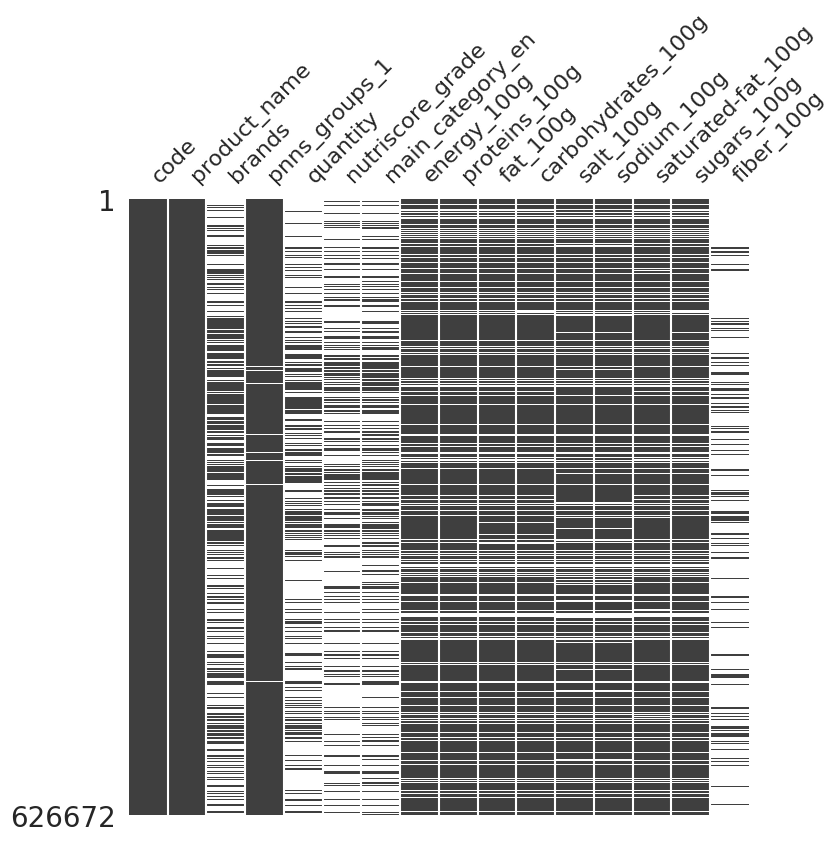
\includegraphics[width=80mm]{completness.png}
      \caption{Taux de remplissage des champs}
      \label{completness}
    \end{figure}
    \subsection{Champs contenant des valeurs textuelles}

    Pour les champs contenant des valeurs textuelles, on traite les champs
    par méthode de <<clustering>>. L'algorithme utilisé est l'algorithme
    de <<Key collision>>.
    (<<StringFingerPrint>> méthode par défaut
    d'OpenRefine\footnote{Le module \Verb"src.utils.string_handler" contient
    également le code nécessaire à une collision de clées par la méthode des
    n-grams.})


\section{Analyses univariées}

  \subsection{Variables sélectionnées}
  Pour assurer la faisabilité du projet, nous avons besoins de :
  \begin{itemize}
    \item Le nom du produit
    \item Le code bar du produit
    \item La marque du produit
    \item La catégorie à la quelle appartient le produit
    \item Le nutriscore (nutrition grade [A, ..., E])
    \item Certaines données nutritionnelles :
    \begin{itemize}
      \item Valeur énergétique au 100g
      \item Teneur en protéines
      \item Teneur en sucres
      \item Teneur en graisses
      \item Teneur en sel
    \end{itemize}
  \end{itemize}


  \subsection{Répartition du nutriscore}
  \begin{figure}[H]
    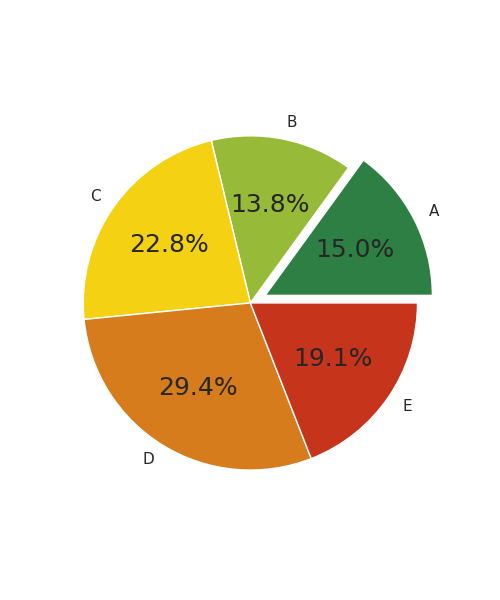
\includegraphics[width=70mm]{nutriscore_pie.png}
    \caption{Répartition du nutriscore des produits}
    \label{nutriscore_pie}
  \end{figure}

  \subsection{Marques, groupes PNNS et catégories}
  \begin{figure}[H]
    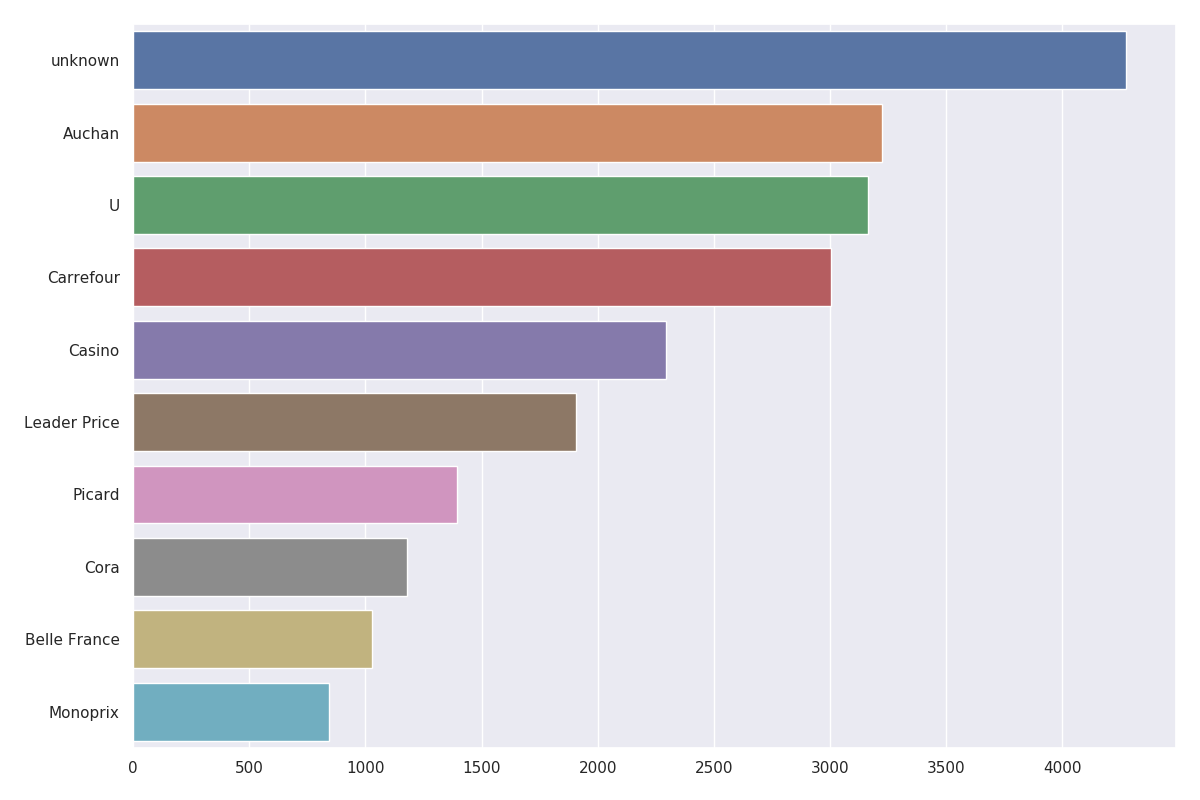
\includegraphics[width=75mm]{brands_repartition.png}
    \caption{Répartion des produits en fonction des marques}
    \label{}
  \end{figure}
  \begin{figure}[H]
    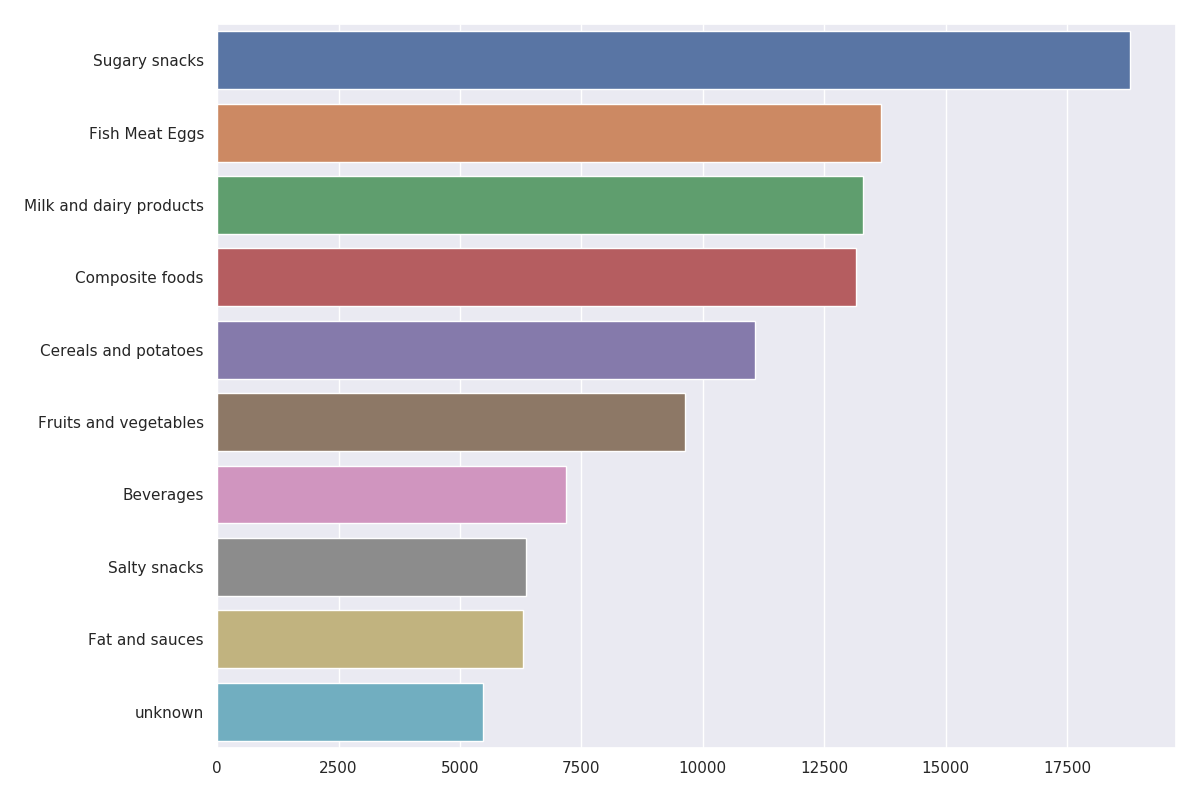
\includegraphics[width=75mm]{pnns_1_repartition.png}
    \caption{Répartion des produits en fonction du groupe PNNS}
    \label{}
  \end{figure}

  \subsection{Catégories}
  voir \textsc{\bf{Figure \ref{wc_cat}}}
  \begin{figure*}
    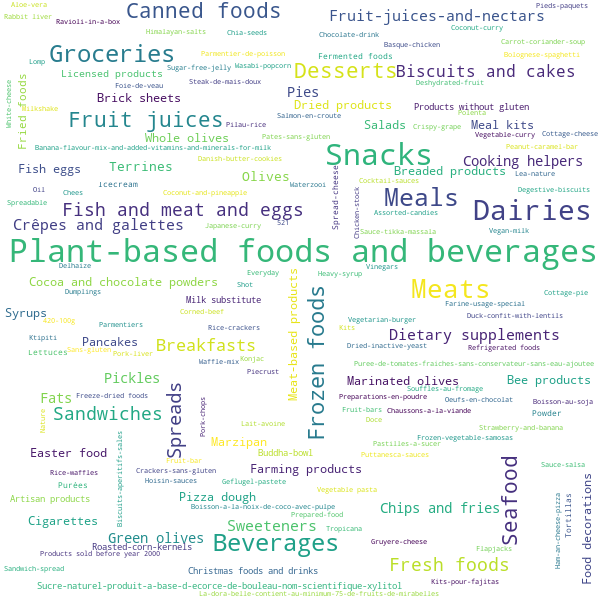
\includegraphics[width=\linewidth]{wc_categories.png}
    \caption{Les catégories présentent dans la base de données sous forme de
    nuage de mot (wordcloud)}
    \label{wc_cat}
  \end{figure*}

  \subsection{Valeurs énergétiques des produits}
  \begin{figure}[H]
    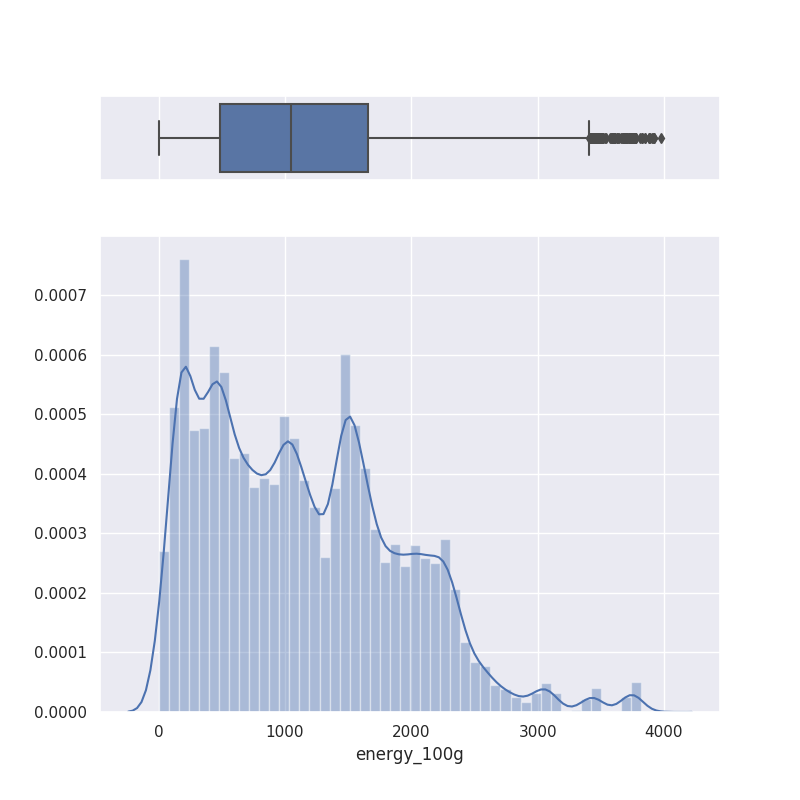
\includegraphics[width=75mm]{energy_100g-dist.png}
    \caption{Distribution des valeurs énergétiques des produits dans la base
    de données.}
    \label{}
  \end{figure}

  \subsection{Nutriments aux 100g}
  \begin{figure}[H]
    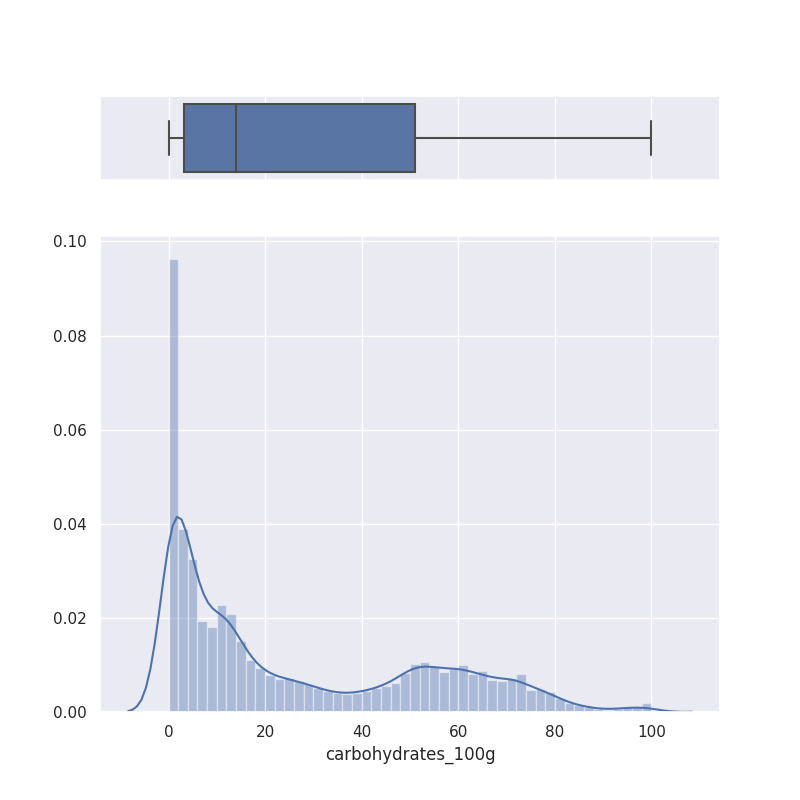
\includegraphics[width=75mm]{carbohydrates_100g-dist.png}
    \caption{Distribution de la quantité de glucides aux 100g}
    \label{}
  \end{figure}

  \begin{figure}[H]
    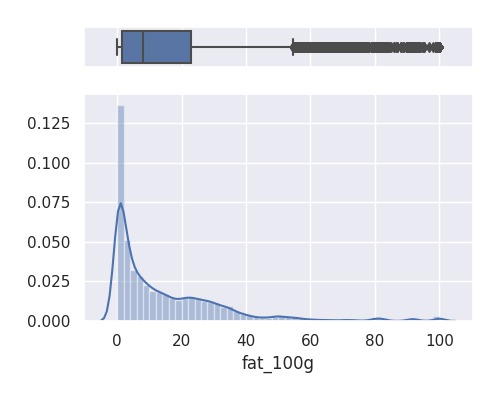
\includegraphics[width=75mm]{fat_100g-dist.png}
    \caption{Distribution de la quantité de graisse aux 100g}
    \label{}
  \end{figure}
  \begin{figure}[H]
    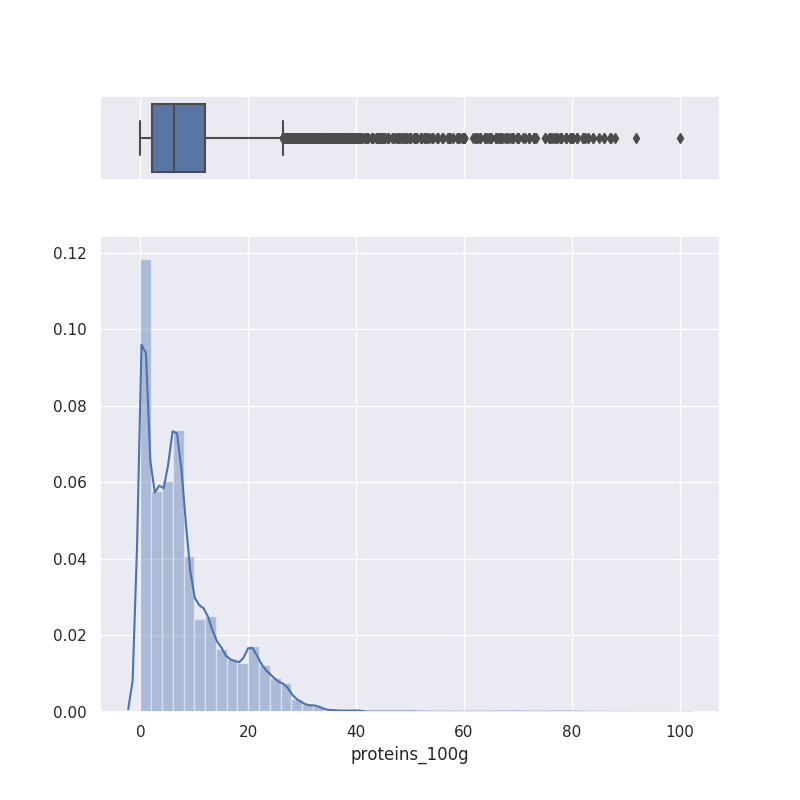
\includegraphics[width=75mm]{proteins_100g-dist.png}
    \caption{Distribution de la quantité de protéines aux 100g}
    \label{}
  \end{figure}


\section{Analyses multivariées}
Toujours dans l'objectif de trouver un produit équivalent, il est important
de vérifier que pour chaque catégorie (ici groupe Programme nutrition santé PNS)
il existe des produits pour chaque nutriscore (de A à E).

  \subsection{Nutriscore et marques}
    \begin{figure}[H]
      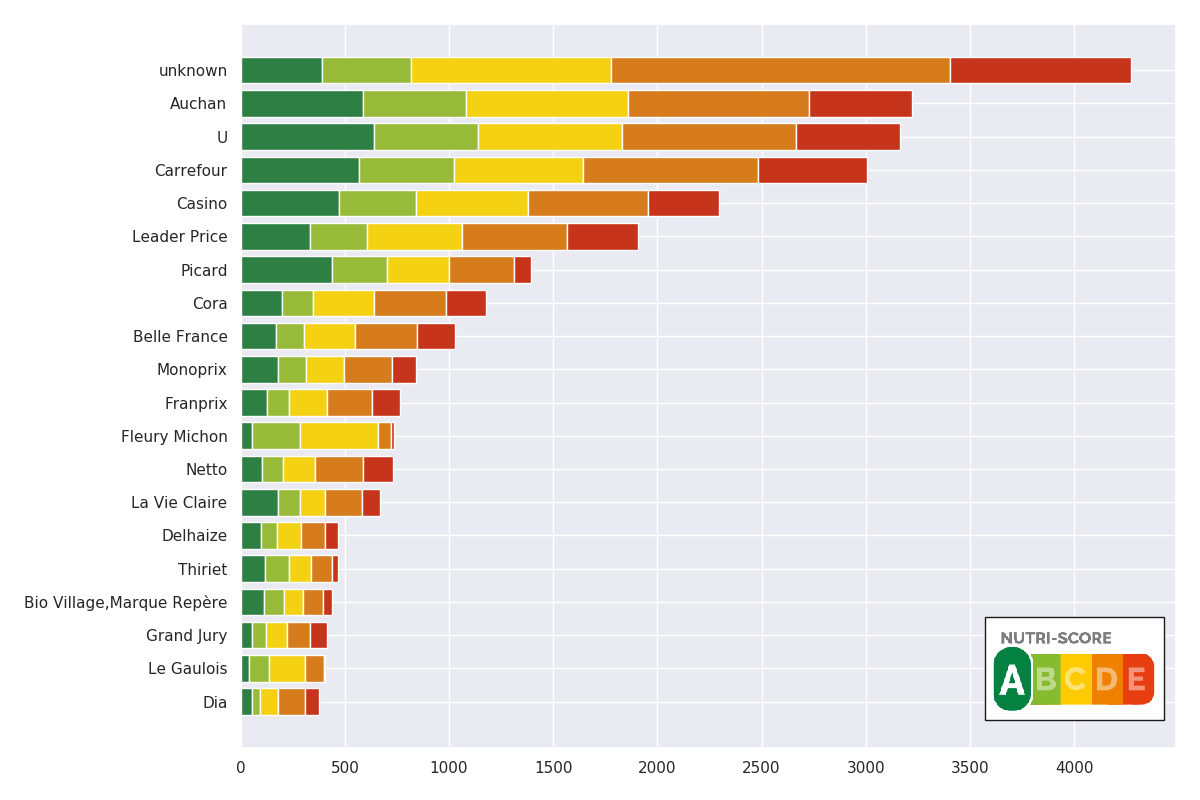
\includegraphics[width=75mm]{brands_nutscore_repartition.png}
      \caption{Repartition du nutriscore au sein des marques}
      \label{}
    \end{figure}
    \begin{figure}[H]
      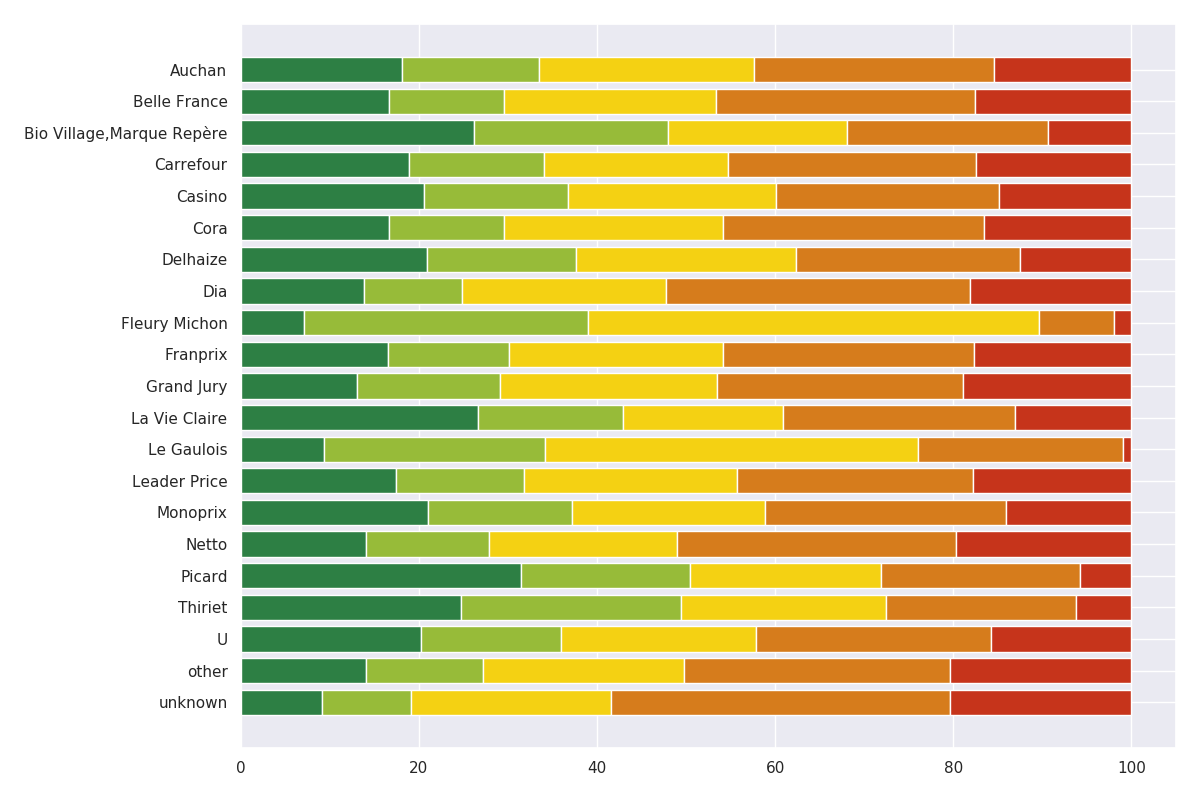
\includegraphics[width=75mm]{brands_nutscore_repartition_freq.png}
      \caption{Repartition du nutriscore au sein des marques (normalisé en fréquence)}
      \label{}
    \end{figure}

  \subsection{Nutriscore et groupes PNNS}
  \begin{figure}[H]
    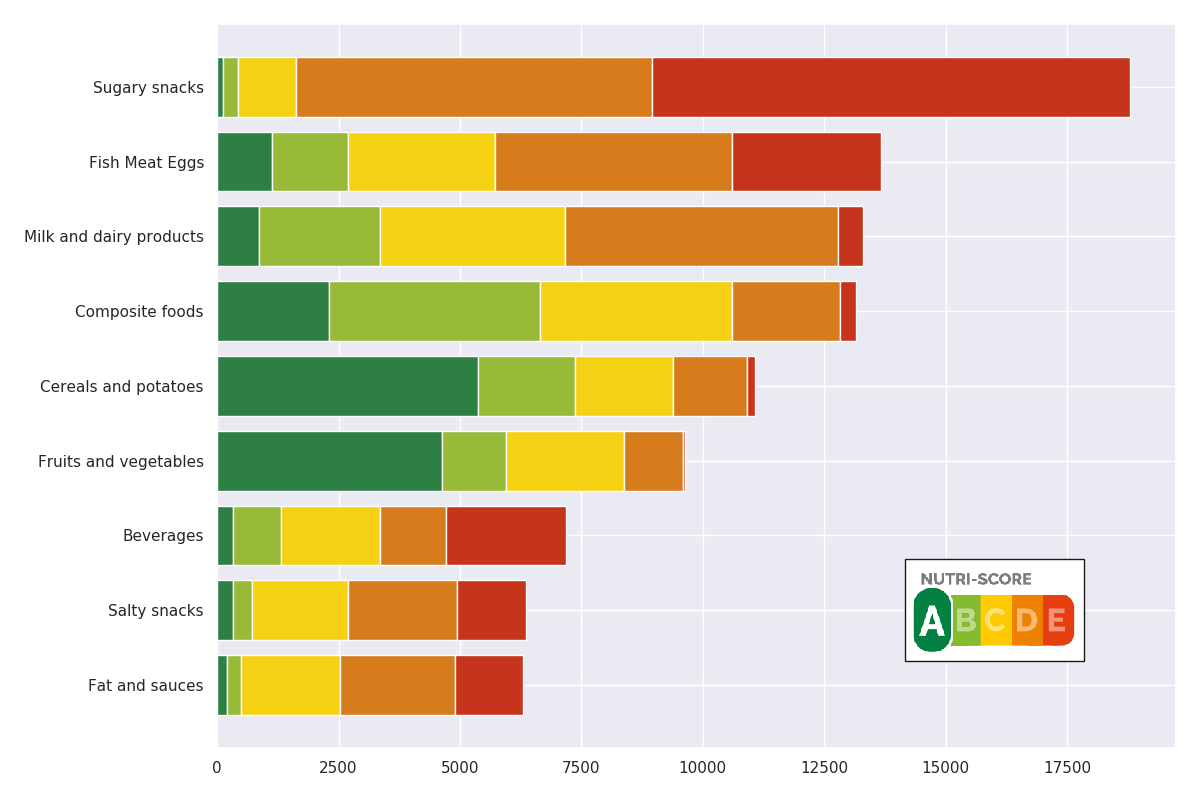
\includegraphics[width=75mm]{pnns1_nutscore_repartition.png}
    \caption{Repartition du nutriscore au sein des groupes PNNS}
    \label{}
  \end{figure}
  \begin{figure}[H]
    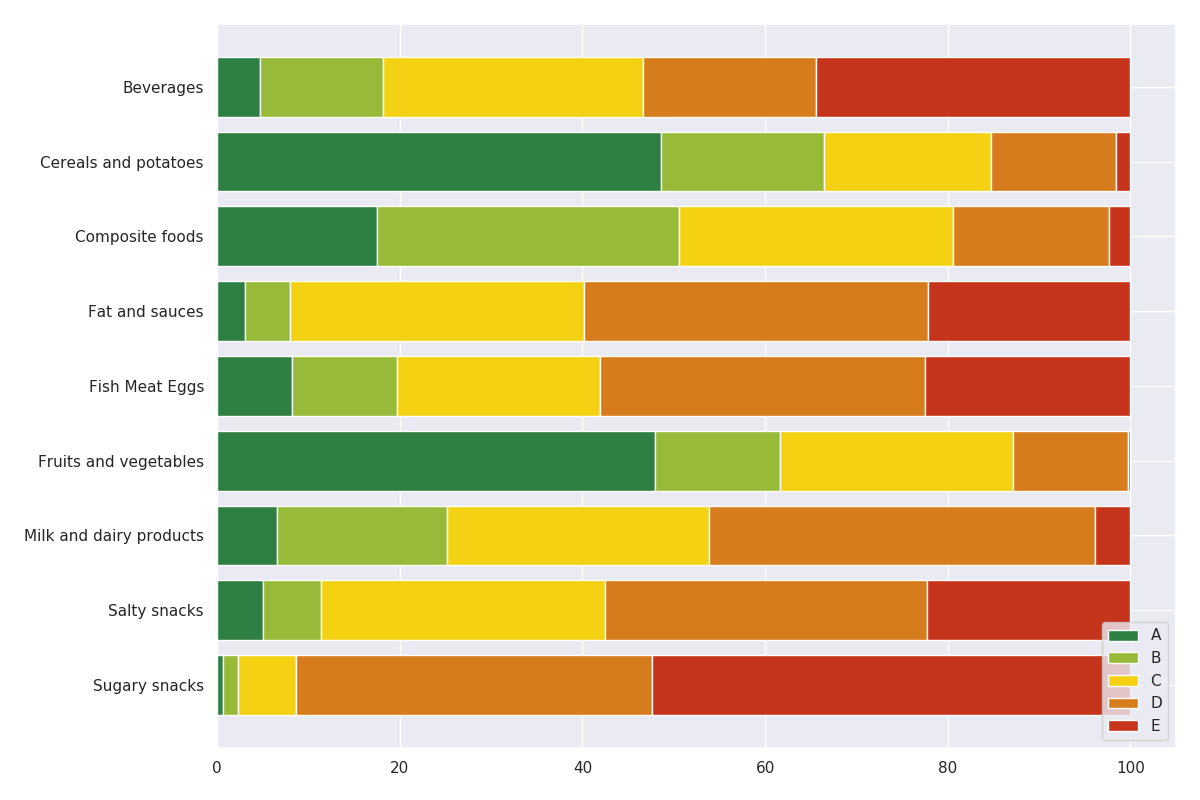
\includegraphics[width=75mm]{pnns1_nutscore_repartition_freq.png}
    \caption{Repartition du nutriscore au sein des groupes PNNS (normalisé en fréquence)}
    \label{}
  \end{figure}

  \begin{table}[H]
    \footnotesize\setlength{\tabcolsep}{2.5pt}
    \caption{Tableau de contingence groupe PNNS et Nutriscore}
    \label{}
    \begin{tabular}{lrrrrr}
\toprule
nutriscore\_grade &      a &      b &      c &      d &      e \\
pnns\_groups\_1           &        &        &        &        &        \\
\midrule
Beverages               &    335 &    972 &   2038 &   1359 &   2473 \\
Cereals and potatoes    &   5375 &   1984 &   2022 &   1520 &    168 \\
Composite foods         &   2303 &   4347 &   3946 &   2239 &    311 \\
Fat and sauces          &    192 &    308 &   2028 &   2367 &   1393 \\
Fish Meat Eggs          &   1121 &   1564 &   3041 &   4874 &   3071 \\
Fruits and vegetables   &   4621 &   1317 &   2449 &   1215 &     27 \\
Milk and dairy products &    871 &   2478 &   3814 &   5615 &    517 \\
Salty snacks            &    319 &    401 &   1981 &   2239 &   1412 \\
Sugary snacks           &    116 &    322 &   1181 &   7337 &   9848 \\
unknown                 &    487 &    737 &   1431 &   2029 &    782 \\
Sum                     &  15740 &  14430 &  23931 &  30794 &  20002 \\
\bottomrule
\end{tabular}

  \end{table}

  \subsection{Valeurs énergétiques des aliments et nutriscore}
  \begin{figure}
    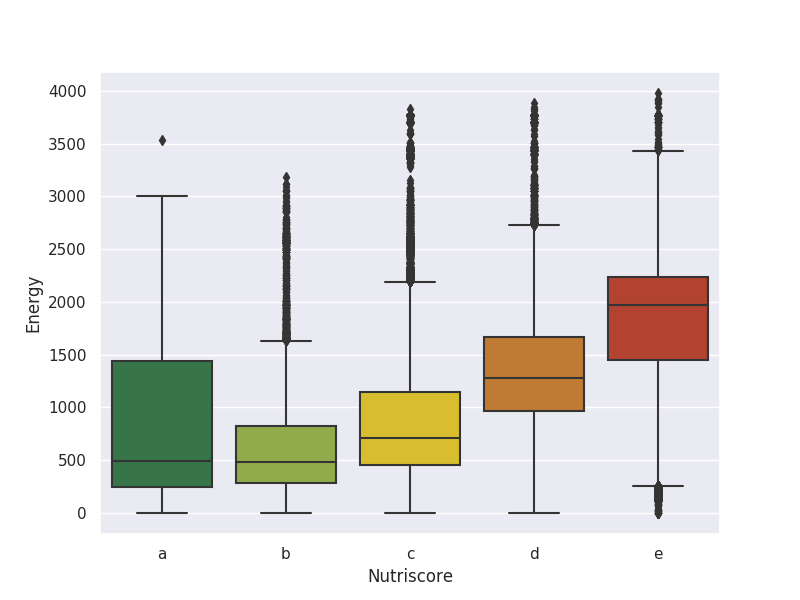
\includegraphics[width=90mm]{box_plot_energy_nutscore.png}
    \caption{}
    \label{}
  \end{figure}

  \subsection{Nutriscore / valeurs énergétiques / composition des produits}


  \begin{figure*}[h]
    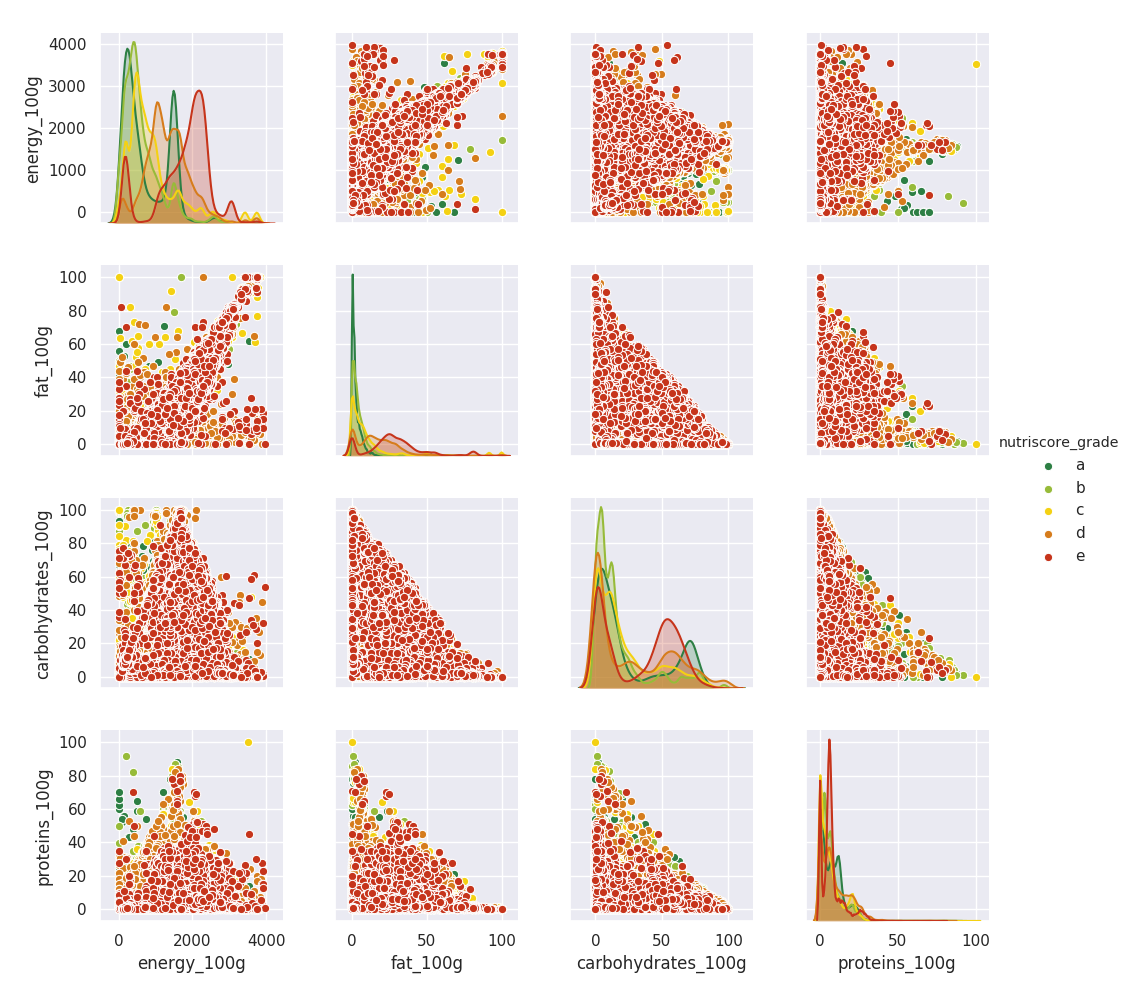
\includegraphics[width=\linewidth]{relational_plot.png}
    \caption{}
    \label{relplot}
  \end{figure*}

  voir \textsc{\bf{Figure \ref{relplot}}}
\section{Conclusion}

\section{Perspectives}

%\section*{Remerciements}

\section{Liens internet}
\label{Liens}
\begin{itemize}
  \item \faGithub \url{https://github.com/tgrandjean/OC-sante-publique-france}
  \item \faDatabase \url{https://world.openfoodfacts.org/data}
  \item \faFileO \url{https://tgrandjean-oc-reports.s3.eu-west-3.amazonaws.com/openfoodfacts/profiling_report.html}
\end{itemize}




%----------------------------------------------------------------------------------------
%	BIBLIOGRAPHY
%----------------------------------------------------------------------------------------

\printbibliography[title={Bibliographie}] % Print the bibliography, section title in curly brackets

%----------------------------------------------------------------------------------------

\end{document}
